\chapter{Creating Variables in Opus}
\label{chap:creating-variables}

Opus is implemented in the Python programming language, so we provide a
review of the language in Appendix \ref{appendix:python}. Numpy is a numerical
library for Python that is used extensively in the Opus system, and is
covered in Appendix \ref{appendix:numpy}. Using Python and Numpy, many of the
Opus Variables are coded as modules (a module is a Python program stored as
a file), and these are explained in Section
\ref{sec:creating-new-variables}.  Finally, a recent and extremely valuable
addition to the Opus architecture is a small language for Opus Expressions,
which makes the need to code variables as separate modules unnecessary in
most cases.  The expression language is the subject of Section
\ref{sec:expressions}.



\section{Opus Expressions}
\label{sec:expressions}
\index{expressions}

Opus uses Python and Numpy to create variables to be used in models.  These are often coded in Python modules as
described in the preceding section.  However, in order to make the use of variables simpler for users to access, a new
\emph{expression language} has been created for Opus
that allows variables to be defined with a relatively simple and concise syntax.  In fact, at this point, many of the variables that
have been previously implemented as modules could be replaces by simpler one-line expressions using this language.

The syntax consists of using Numpy operations and methods, operating on Opus variables and primary data.  All of the Numpy operators are available, and work in the same way for expressions, including \verb#+ -  * / **#, where ** is an exponential function: a**3 returns a to the power of 3.

Expressions allow an \verb#alias#, or name, to be assigned to the expression, in order to use it by this reference in a model specification or indicator function.  The standard syntax in Opus uses short names, with lower case letters.  If two or more words are used in a name, we usually separate the components with an underscore to make the name more readable.  Some examples will illustrate key aspects of the expression syntax:

\begin{itemize}

\item \code{hwy\_300 = gridcell.distance\_to\_highway<300} would generate a dummy variable equal to 1 for gridcells that have an attribute value of distance to highway less than 300 meters.  Note that in this case we are operating on a \verb#primary attribute# of gridcells, which means that it is part of the data that we initially load into the model, as opposed to data we compute within the model.

\item \code{ln\_pop = ln(urbansim.gridcell.population} would be used to compute the log of an existing variable, population, which is in the urbansim package and applies to the gridcell dataset.

\item \code{pop\_emp\_ratio = urbansim.gridcell.population / urbansim.gridcell.number\_of\_jobs} would compute the ratio of population to employment, using variables stored in the urbansim package, associated with the gridcell dataset.  

\end{itemize}

Two very useful methods in the expression language are \verb#aggregation# and \verb#disaggregation#.  Aggregation allows an expression to compute a result on one dataset and aggregate the results to assign to another dataset, such as summing the population in households that live in a gridcell.  Using this expression approach, we could replace the long population.py module in the preceding section with the following expression:

\code{population = gridcell.aggregate(household.persons)}

That is quite a lot easier to understand and to code!  We are aggregating to the gridcell dataset, from the household dataset, the number of persons.  However, in the time since the variable in the preceding section was implemented, we have changed the data structure for the gridcell and parcel based models to use buildings.  So now, households and jobs are associated with buildings, and buildings are associated with gridcells (or parcels).  This means that in order to compute the population of a gridcell, we need to first aggregate it to building, and then from building to gridcell.  That is not hard to do, either, by simply adding an intermediated argument to the aggregation function.  There can be multiple levels of intermediates, if needed:

\code{population = gridcell.aggregate(household.persons, intermediates = [building])}

The default method for aggregation is to sum, but there are several other aggregation methods available also:

\squishlist
\item sum
\item mean
\item maximum
\item mininim
\item variance
\item standard\_deviation
\item center\_of\_mass
\squishend

To use any of these functions, we simply add \verb#function = mean# (or another function) in the expression.  Here is an example to determine the average household size per gridcell:

\code{avg\_hhs = gridcell.aggregate(households.persons, intermediates = [building], function = mean)}

The \verb#disaggregate# method for expressions assigns values from one dataset to another, in a one to many relationship.  In other words, it works in the opposite direction from the aggregate method, which is many to one.  An example would be to assign the zonal population density to all households living the zone.  In this example, we use the \verb#population_density# variable in the zone dataset of the urbansim\_parcel package, and assign it to households, which are connected to zones indirectly through buildings and then parcels: household -$>$ building -$>$ parcel -$>$ zone.  So the expression would be:

\code{density = household.disaggregate(urbansim\_parcel.zone.population\_density, intermediates = [building, parcel])}

Note that for both aggregate and disaggregate methods, the first element, preceding the method name, is the name of the dataset to which the result should be assigned.  zone.aggregate... should generate some result and assign it to zone, whereas gridcell.disaggregate... should assign some value from a larger geography to the gridcell dataset.

A list of expressions can be stores in an \verb#aliases.py# file within a package and dataset directory.  This provides an efficient means to organize and store many expressions in a single location.  Below are some of the aliases in the urbansim\_parcel/parcel/aliases.py module that demonstrate some of the expressions in actual use in the model system.\\

%\begin{lstlisting}
"used_land_area = (parcel.aggregate(building.land_area, function=sum)).astype(int32)",
"vacant_land_area = parcel.parcel_sqft - urbansim_parcel.parcel.used_land_area",
"unit_name = parcel.disaggregate(land_use_type.unit_name)",
"building_sqft = (parcel.aggregate(urbansim_parcel.building.building_sqft)).astype(int32)",
"building_sqft_per_unit = safe_array_divide(urbansim_parcel.parcel.building_sqft, urbansim_parcel.parcel.residential_units)",
"residential_units = (parcel.aggregate(building.residential_units)).astype(int32)",       
"parcel_sqft_per_unit = safe_array_divide( parcel.parcel_sqft, (urbansim_parcel.parcel.residential_units).astype(float32) )",
"unit_price = safe_array_divide(parcel.land_value + urbansim_parcel.parcel.improvement_value, urbansim_parcel.parcel.existing_units)",
"demolition_cost = (parcel.aggregate(urbansim_parcel.building.demolition_cost)).astype(int32)",
"improvement_value = (parcel.aggregate(building.improvement_value)).astype(int32)",
"total_value_per_sqft = safe_array_divide(parcel.land_value + urbansim_parcel.parcel.improvement_value, parcel.parcel_sqft)",
"number_of_jobs = parcel.aggregate(urbansim_parcel.building.number_of_jobs)",
"employment = parcel.aggregate(urbansim_parcel.building.number_of_jobs)",
"number_of_households = parcel.aggregate(urbansim_parcel.building.number_of_households)",
"population = parcel.aggregate(urbansim_parcel.building.population)",
"travel_time_to_cbd = parcel.disaggregate(gridcell.travel_time_to_cbd)",       
%\end{lstlisting}

\section{Opus Indicators}
\label{sec:opus-indicators}

Indicators are typically considered summary measures used for
evaluation purposes, like a cost-benefit ratio, or a VMT per capita
measure.  Indicators can also be used for evaluation purposes.  Opus
has a fairly extensive infrastructure for computing indicators.  Some
of it is already available in the new Opus GUI, but there is more
functionality available using scripts.  In the eugene package, for
example, there is an indicators directory containing a
make\_indicators.py script that demonstrates the use of a script to
make a series of different kinds of indicators.  
% A more extensive set
% of examples and documentation is provided in the script 
% /opus/src/opus\_core/indicator\_framework/make\_indicators\_example.py.

Indicators generally use expressions to do their computation, so they
share all of the functionality described in the preceding section.  The
Opus Indicator Framework, however, adds some very helpful methods to
also visualize the results of the indicator computation, or to export
the results to a text file, or a table in a database, or to a GIS for
visualization.

The indicator output options currently include the following types:

\squishlist 
\item \emph{Map}: produces a map of the indicator rendered
in Matplotlib. 
\item \emph{Chart}: produces a simple line chart, useful for tracking
an aggregate indicator over multiple years of a simulation. 
\item \emph{Table}: produces a browsable table that can also be
exported, containing two columns: the column containing the level of geography or
aggregation, and the column containing the indicator value for that
aggregation.  A zone table of total population would be an example of
this form. 
\item \emph{DatasetTable}: produces a table with multiple
indicators for the same unit of aggregation or geography, such as
employment by zone, with multiple columns representing the total
employment for each industry sector, and possibly other indicators.  It
would contain one record per zone. 
\squishend

The Opus GUI currently supports all these output types except the
chart. The following tutorial focuses on the use of the GUI to
create and visualize several different kinds of indicators.

Assume that we want to run the eugene\_gridcell baseline scenario from
1980 to 1990, and then will generate the following indicators from the
simulation results:

\squishlist
\item Average cars per household by gridcell, viewed as a map
\item Average cars per household by zone, viewed as a map
\item Average household size per zone, viewed as a table
\item Log of the sum of population and employment by gridcell, as a map
%\item Total population by zone, as a table
\squishend

For the first indicator, we need an expression that would compute the
average number of cars for the households living in a gridcell, and
then to display this on a map.  The expression is straightforward:

\code{cars\_per\_hh = gridcell.aggregate(household.cars, function=mean)}

Note that since we are operating on a \verb#primary attribute# of the
data (we can find \verb#cars# in the data directory under
data/eugene\_gridcell/household), we do not need to put a package name
in the expression.  We could leave out the alias \verb#cars_per_hh =#,
but when we generate the indicator and map, using an alias will provide
a meaningful default title on the Matplotlib map.

Make sure that you have run a
simulation on the computer you are using (see
Chapter~\ref{chap:scenarios-manager}) that has run over multiple
years. Create the \verb#cars_per_hh# indicator (creating a new
indicator in the GUI is covered in
Chapter~\ref{chap:variable-library}). You can visualize the result
by following the directions in
Section~\ref{sec:interrogating-results-with-indicators}. You
will see something like that shown in
figure~\ref{fig:indicator-cars-gridcell-2}.

% \begin{figure}[htp]
% \begin{center}
% 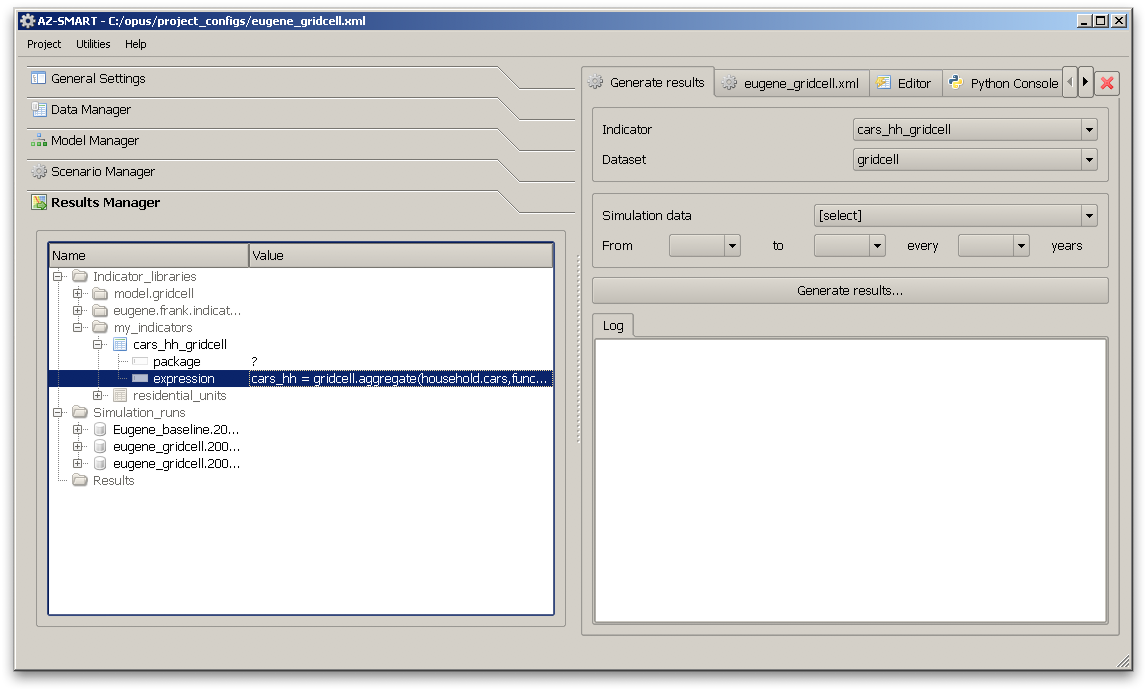
\includegraphics[scale=0.4]{graphics/indicator-cars-gridcell-1.png}
% \end{center}
% \caption{Generating the Average Cars per Household in a Gridcell}
% \label{fig:indicator-cars-gridcell-1}
% \end{figure}

\begin{figure}[htp]
\begin{center}
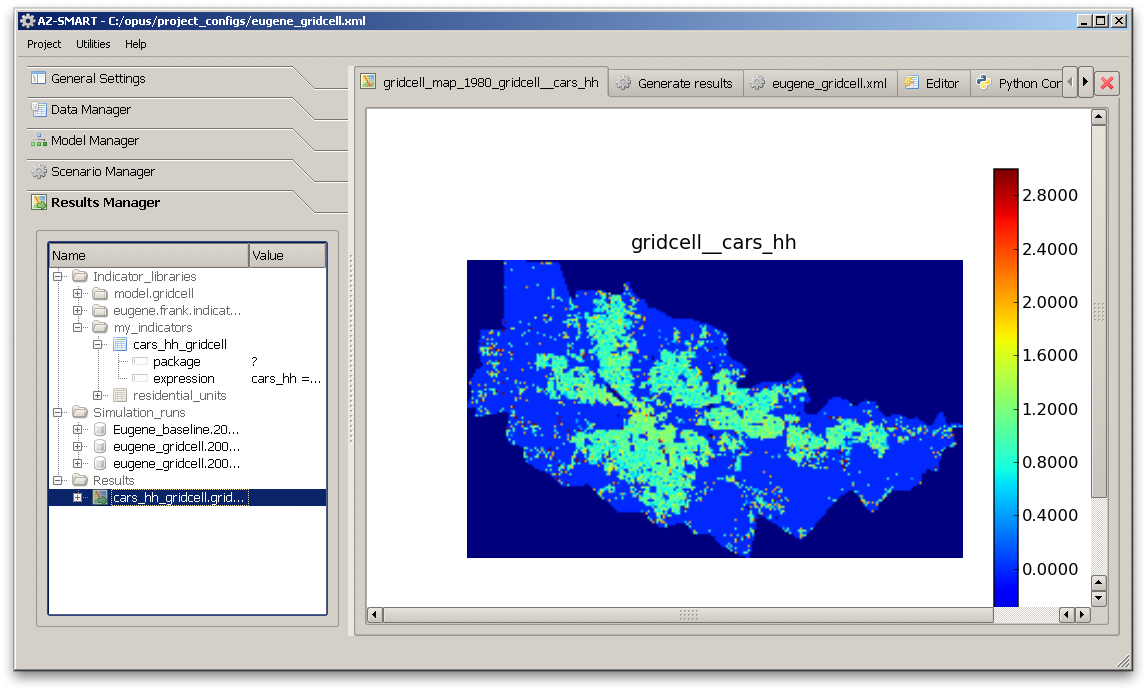
\includegraphics[scale=0.4]{graphics/indicator-cars-gridcell-2.png}
\end{center}
\caption{Generating the Average Cars per Household in a Gridcell}
\label{fig:indicator-cars-gridcell-2}
\end{figure}

In order to compute the second indicator, we will need to average the
number of cars per household at the zonal level as follows:

\code{cars\_per\_hh = zone.aggregate(household.cars, intermediates= [gridcell], function=mean)}

% T: this is actually not true, it works just fine
% The only remaining problem with this is that we cannot display zonal
% data using Matplotlib, which generates only raster image maps, meaning
% that it only supports displaying data assigned to gridcells.  Recalling
% the \verb#disaggregate# function in the expression language, we can
% just disaggregate the zonal average like this:
% 
% \code{cars\_per\_hh = gridcell.disaggregate(zone.aggregate(household.cars, intermediates= [gridcell], function=mean))}

To generate the third indicator of average household size we could use
a similar expression:

\code{persons\_per\_hh = zone.aggregate(household.persons, function=mean, intermediates = [gridcell])}

Now we use a compound expression, to sum the result of two variables,
and take the log of the result.  This is to produce the indicator as
shown below:

\code{ln\_emp\_pop=ln(urbansim.gridcell.population+urbansim.gridcell.number\_of\_jobs)}

Note that these are variables which can be found on the disk in
src/urbansim/gridcell.  The result of visualizing this indicator is
shown in Figure \ref{fig:indicator-ln-emp-pop}.

\begin{figure}[htp]
\begin{center}
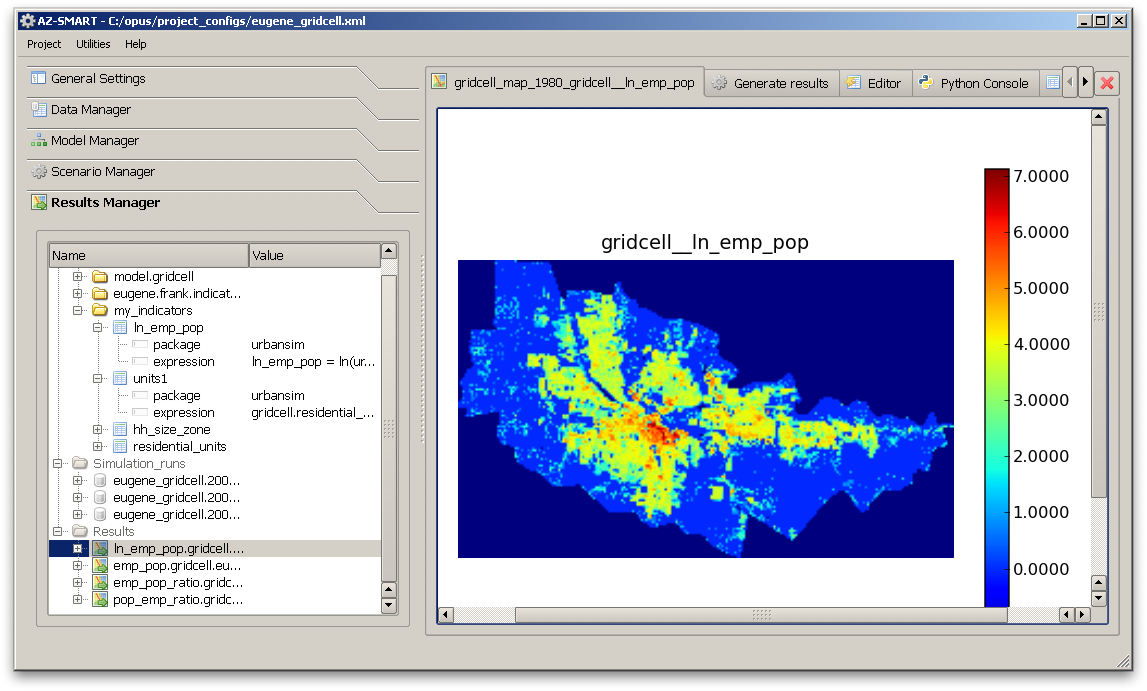
\includegraphics[scale=0.4]{graphics/indicator-ln-emp-pop.png}
\end{center}
\caption{Log of (Population + Employment) by Gridcell}
\label{fig:indicator-ln-emp-pop}
\end{figure}

% For the last indicators in the list to be done, we return to
% indicators that are already defined in a generic indicator library in
% the results manager.  To produce the population by zone indicator and
% visualize it as a table, use the following steps.  Right-click on the
% population indicators, and select \verb#Generate results with#.  In the
% form that is created on the right, select the pull-down menu labeled
% \verb#Dataset# and click on zone.  This is a generalized indicator that
% uses a simple mechanism to allow different levels of aggregation to be
% selected in this way, without the need to type in an expression as was
% done in the preceding examples.  Select a simulation result, and
% generate the indicator.  Then select the new indicator result
% containing the indicator values, right-click, and select \verb#View
% result as# and choose \verb#Table#.  This should generate a browsable
% table in the form window, as shown below in Figure
% \ref{fig:indicator-population-zone-table}.
% 
% \begin{figure}[htp]
% \begin{center}
% 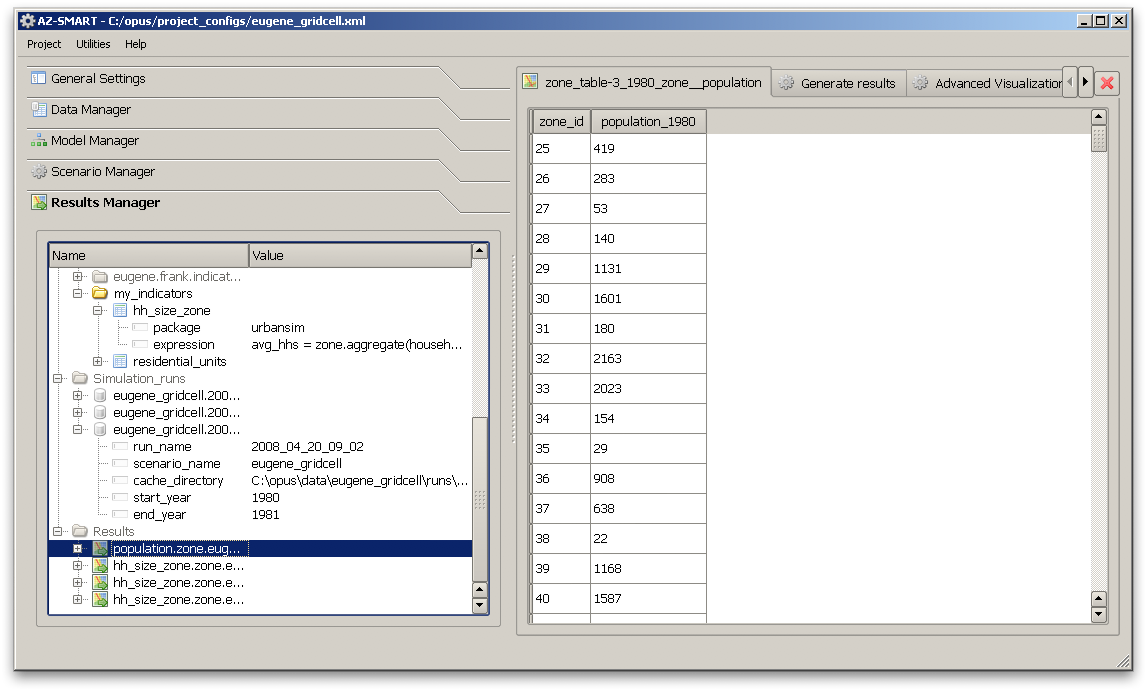
\includegraphics[scale=0.4]{graphics/indicator-population-zone-table.png}
% \end{center}
% \caption{Viewing the Population by Zone Indicator as a Table}
% \label{fig:indicator-population-zone-table}
% \end{figure}
% 
% Now that we have seen the integrated Matplotlib maps, you might want to
% know how to export an indicator to a more full-featured GIS system such
% as ArcGIS (a commercial package from Environmental Systems Research
% Institute), or PostGIS (an open source package built on the Postgres
% database).  The Results Manager is now able to export a table with one
% or more indicators to an ESRI Geodatabase for further analysis and
% visualization.  In the following example, we export the same indicator
% result shown above as a table, to an ESRI File-based Geodatabase. 
% Other Geodatabase formats are also supported.
% 
% If the population by zone table result is still available, right-click
% on the result in the tree on the left-hand side of the window, and
% select the \verb#View result as# and choose \verb#Advanced
% visualization#.  It will generate a form as shown in Figure
% \ref{fig:indicator-population-zone-export}.  We need to add the
% indicator we have generated to the set, in the upper portion of this
% form, and select the location of the ESRI geodatabase.  I am assuming
% that the geodatabase contains a \verb#Feature Class# corresponding to
% the table being exported. In this example, the table corresponds to the
% zone feature class.  Once the form is filled in, click on the
% \verb#Go!# button, to start the export process.  A message will be
% printed to the log to indicate the completion status of this export
% process.
% 
% \begin{figure}[htp]
% \begin{center}
% 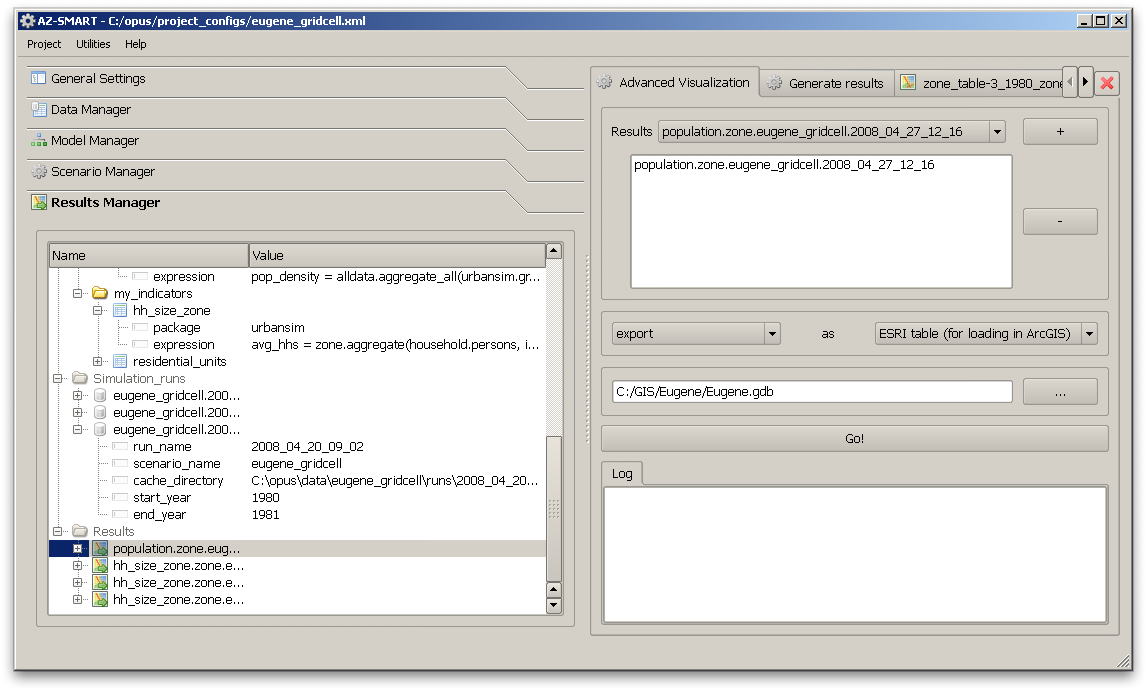
\includegraphics[scale=0.4]{graphics/indicator-population-zone-export.png}
% \end{center}
% \caption{Exporting the Population by Zone Indicator to an ESRI Geodatabase}
% \label{fig:indicator-population-zone-export}
% \end{figure}
% 
% Once the export is successfully completed, the geodatabase will contain
% a table that contains the indicator result, with a zone\_id and an
% ArcGIS \verb#OBJECTID*# that corresponds to the internal object ids in
% the feature class.  It is safe to join the indicator table result with
% the feature class using either the objectid or the zone\_id.  The map
% in Figure \ref{fig:indicator-population-zone-arcgis} shows the result
% of joining the feature class with the indicator table and generating a
% thematic map of the populaion by zone, using the zone.acres field to
% normalize the population, resulting in a map of population density per
% acre.
% 
% \begin{figure}[htp]
% \begin{center}
% 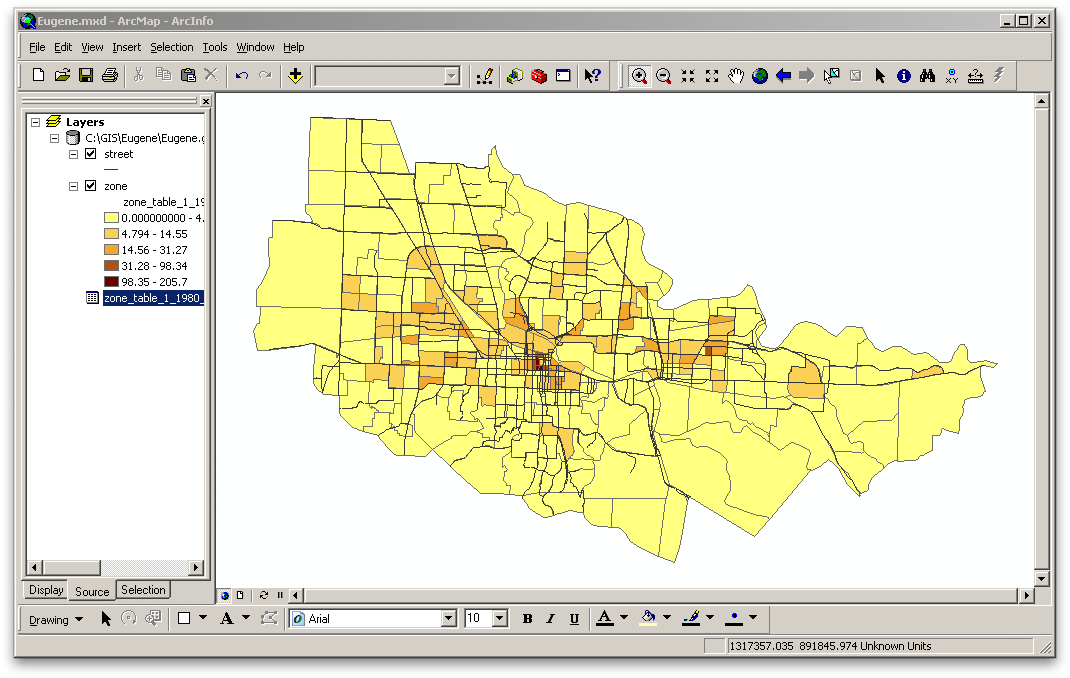
\includegraphics[scale=0.4]{graphics/indicator-population-zone-arcgis.png}
% \end{center}
% \caption{Mapping the Population by Zone Indicator in ESRI ArcMap}
% \label{fig:indicator-population-zone-arcgis}
% \end{figure}

\section{(advanced) Creating New Opus Variables}
\label{sec:creating-new-variables}

Variables in Opus are Python modules containing a single Python
\verb#Class# that computes a variable and returns the result.  For
demonstration purposes, the population variable in
\verb#/src/urbansim/gridcell/population.py# is shown below.  We refer
to a variable using a \verb#Pythonpath#, which provides a means for
Python to find modules and classes in a directory structure.  So, a
reference to this particular module using a \verb#fully qualified path#
would be \verb#urbansim.gridcell.population#.  You can find all of the
existing variables by browsing on disk in the source code directory. 
The directory structure mirrors the parts of the variable name, so that
urbansim.gridcell.population is really pointing to
/opus/src/urbansim/gridcell/population.py, which is included below as
an example.

\begin{lstlisting}
from opus_core.variables.variable import Variable
from urbansim.functions import attribute_label
from variable_functions import my_attribute_label
from opus_core.logger import logger

class population(Variable):
    """Compute the total number of people residing in a gridcell, 
    by summing hh_persons over all households in the gridcell"""
    
    _return_type="int32"
    hh_persons = "persons"

    def dependencies(self):
        return [attribute_label("household", self.hh_persons), 
                attribute_label("household", "grid_id"), 
                my_attribute_label("grid_id")]

    def compute(self, dataset_pool):
        households = dataset_pool.get_dataset('household')
        return self.get_dataset().sum_dataset_over_ids(households, self.hh_persons)


from opus_core.tests import opus_unittest
from opus_core.tests.utils.variable_tester import VariableTester
from numpy import array
class Tests(opus_unittest.OpusTestCase):
    def test_my_inputs(self):
        gridcell_grid_id = array([1, 2, 3])
        #specify an array of 4 hh's, 1st hh's grid_id = 2 (it's in gridcell 2), etc.
        household_grid_id = array([2, 1, 3, 2]) 
        #specify how many people live in each household
        hh_persons = array([10, 5, 20, 30])

        tester = VariableTester(
            __file__,
            package_order=['urbansim'],
            test_data={
                "gridcell":{
                    "grid_id":gridcell_grid_id 
                    }, 
                "household":{ 
                    "household_id":array([1,2,3,4]),
                    "persons":hh_persons, 
                    "grid_id":household_grid_id
                }
            }
        )
        
        should_be = array([5, 40, 20])
        tester.test_is_close_for_family_variable(self, should_be)

if __name__=='__main__':
    opus_unittest.main()
\end{lstlisting}

Some new features presented in this example are the use of a Python Class, which is a topic I will defer for now, the use of dependencies (other variables or primary attributes of datasets that the current variable depends on), and the use of tests in code to ensure that the computation is doing what is expected.  The use of Python modules containing a Class to compute a single variable is flexible and quite powerful, but a bit too complex for most users to use on a regular basis, especially if what is desired is a simple transformation of an attribute or a variable.  Until recently, even something as simple as taking the logarithm of this population variable would have required writing a new module to to that transformation.  Fortunately, this is no longer necessary, since a new Opus Expression language has been implemented.
